\documentclass[12pt]{article}
\usepackage[margin=1in]{geometry}
\usepackage[style=numeric,sorting=none,maxnames=3]{biblatex}
\usepackage{libertine}
\usepackage{graphicx}
\usepackage{inconsolata}
\urlstyle{same}
%\setlength{\parindent}{0pt}
\addbibresource{references.bib}

\linespread{2}
\renewcommand{\maketitle}{%
	\begin{center}
		\textbf{\Large{King Minos: The Father of Heavenly Law}}\\
		\vspace{1.5cm}
		AGRS 28 Term Paper\\
		Yutong Du\\
		GSI: Rebekah McKay, Fridays 1-2pm
	\end{center}
}

\title{King Minos: The Father of Heavenly Law}
\author{Yutong Du}
\date{\today}
\begin{document}
	\begin{titlepage}
		 \vspace*{\fill}
		\maketitle
		 \vspace*{\fill}
	\end{titlepage}	
	\pagebreak
	\begin{center}
		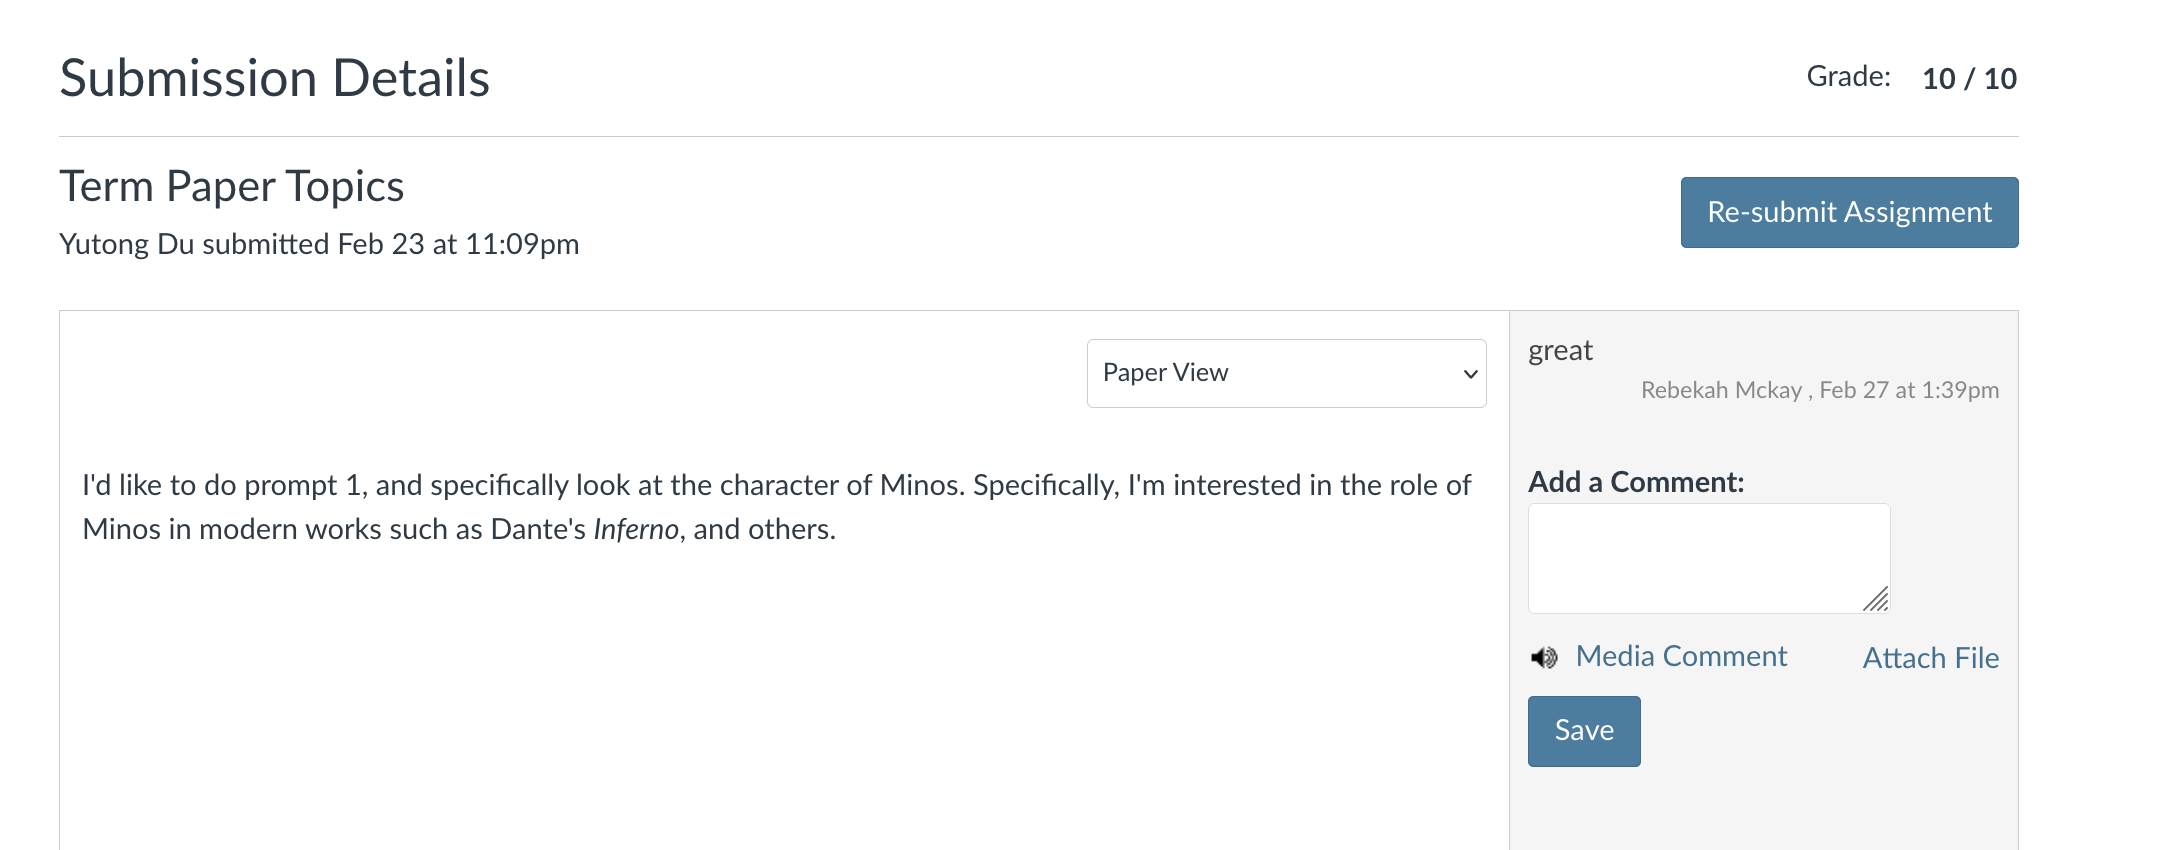
\includegraphics[scale=0.4]{term-paper.png}
	\end{center}
	\pagebreak

	One of the most important figures in mythology in regards to order within society is 
	King Minos, son of Zeus and Europa. In mythology, he is most well known for being the king of Knossos, a city 
	located on the island of Crete, and is also well known for his conversations with Zeus to bring 
	laws to the land below. While references of Minos in mythology are really limited to only a few select myths, 
	his legacy as a lawmaker and the myths he's a part of have had a lasting impact on several significant  
	works in contemporary works. 

	Within mythology, perhaps \textit{the} most famous myth in which Minos appears is that of Theseus and the Minotaur.
	As the myth goes, Theseus grows up in Troezen and arrives in Athens, where he learns of the punishment 
	given to the Athenians -- every year, the city must surrender fourteen children (seven boys and seven girls) 
	to face the minotaur, a half-human, half-bull that resides within the Labyrinth built by Deadalus. This minotaur 
	is intimately connected to Minos, as it is the product of the divine punishment Poseidon exacted upon the king, for 
	not sacrificing the snow-white bull to him. Specifically, he had Minos's wife Pasipha\"{e} fall in love with the 
	bull, thus giving birth to the Minotaur. Minos then had Deadalus construct a labyrinth to entrap the bull, 
	and later when Minos defeated Athens in conflict, began demanding for sacrifices to it.

	Upon learning of these sacrifices, Theseus volunteers as one of them, and travels to Knossos to face the 
	minotaur himself. Once there, he was ``well received by King Minos" (Seltman 1953, 2), and Minos's daughter, 
	Ariadne also falls in love with Theseus. Knowing that he is about to be sent into the labyrinth, Ariadne gives 
	Theseus a ball of thread, allowing him to retrace his path to the entrance after slaying the minotaur. Theseus 
	does just that, and subsequently elopes with Ariadne, and this is where the relevance to Minos ends. 

	In terms of the plot, Minos really only serves as a catalyst and one of many adversaries Theseus ends up 
	journeying on in order to become recognized as a staple hero in mythology. This is significant, since it highlights 
	that in the grand scheme of things, Minos's role in this story is relatively minor -- Theseus's journey 
	continues without the mention of Minos, highlighting his role as a one-time hurdle and nothing more.   

	Alongside this myth with the minotaur, Minos also appears in the \textit{Odyssey}, where he is 
	said to have ``conversed with great Zeus" every nine years, and it is from these conversations that he ``brought 
	back laws fore the cities" (Levaniouk 2011, Chapter 5). This passage is significant, because it succinctly 
	summarizes why we associate Minos so heavily with divine law in modern (i.e. anything preceding the Greek 
	and Roman era) times. The nature of these conversations being implied to be the source for the laws 
	of the land highlights not only Minos's connection to divine law, but it also accentuates Minos's importance 
	as a figure in Greek mythology, as this responsibility of passing down the law of the gods demonstrates
	that he is far from any ordinary king. 

	%this paragraph probably doesn't really belong here
%	These two works, along with Plutarch's \textit{Theseus}, mark the two different ways that 
%	Minos is typically depicted within mythology. At times, he's depicted to be a ``harsh and tyrannical ruler,''
%	as is the case with the former myth of Theseus, 
%	but other times he's praised for being `` `amazing' and `hyperbolic,' '' (Lewis 2006, 45)
%	as is the case with the latter account in \textit{Odyssey}. This is an aspect I will come back to later, when 
%	I discuss the relationship between Minos's seemingly conflicting portryal and law itself. In particular, 
%	these two works serve to highlight the harshness, but also the necessary nature of law.  

	In terms of roles in major myths, as far as I can tell, this is where the road ends -- there aren't any other 
	\textit{extremely} notable instances where Minos appears, perhaps he makes a minor appearance in other 
	myths relating to his children, but never again does Minos take the central pedestal as he does 
	in these two myths I've just discussed. However, despite this 
	relatively limited scope, Minos's legacy has made him almost synonymous with divine law in many works that 
	later incorporate the character. One such case of this is in one of Plato's dialogues, titled \textit{Minos}. 
	Firstly, it's obvious that this work is related to king Minos in some way; after all, the entire dialogue is 
	effectively named after him, so already this highlights his importance as a mythological character as he's 
	important enough that Plato has dedicated an entire dialogue to him. More importantly, however, are the contents 
	of this work. The dialogue revolves around Socrates and an unnamed companion debating about law itself, opening
	with the question of ``what is law?'', and exploring the ``limits of law" itself (Lutz 2010, 992). Throughout 
	the second half of the dialogue, Socrates propels the idea of Minos being a symbol of divine justice, by 
	explaining how Minos learned ``whole kingly art" from his conversations with Zeus, then proceeded to 
	``use this art [to] make divine laws that teach virtue and bring happiness." (Lutz 2010, 998). To start, 
	the characterization of the laws as a ``whole kingly art" highlights the immense value Socrates, and therefore 
	Plato holds to the laws Minos passes down, and furthers the synonymity between Minos and the notion of divine law.
	Further, Socrates also explicitly points to Minos's conversations with Zeus as the ``evidence for the divinity 
	of Minos and his laws,'' claiming that Minos was ``the king of Knossos and the confidant of great Zeus'' 
	(Lutz 2010, 999). This explicit connection Socrates draws by labelling Minos as Zeus's ``confidant'' indicates
	to the reader that Minos's status is nearly equal to that of a god, and given this elevated status, further 
	solidifies the notion that the laws he passes down are divine, and are hence of the utmost importance.  

	In addition to placing Minos on this divine pedestal, Socrates also uses the example of Minos to highlight 
	the philosophical dilemma surrounding the creation of law itself. For instance, aside from 
	defining what law is, one of the other central questions \textit{Minos} asks surrounds the creation of 
	law itself -- specifically, whether an ``ideal legislator'' exists (Mulroy 2007, 122). Within the dialogue, 
	Socrates uses Minos as an example of divine law passed down from the gods, and contrasts this with 
	the example of Hipparchus, who ``seeks wisdom from his own invention and readings'' (Mulroy 2007, 122). This 
	contrast is then used to ask the question of ``whether god or some man deserves credit for [the creation 
	and dissemination of] laws." (Mulroy 2007, 122). At the end of it all, both Socrates and the companion 
	agree that neither of them can reasonably be deemed the ideal legislator. (Mulroy 2007, 122)
	The use of Minos within this dialogue exemplifies perfectly 
	the way Minos is portrayed in contemporary works, as he is being used here as a prime example of divine law.
	Further, the deep philosophical question that's being asked as a result of this contrast also serves to
	highlight the importance of Minos in modern society, as the question of legal authorship and the limitations 
	explored in this work remain central to legal philosophy today. 

	Furthermore, another incredibly famous work that Minos appears in is Dante Alighieri's \textit{Divina 
	Commedia} (Divine Comedy). Within the comedy, it is well known that Dante doesn't shy away from incorporating 
	historical Greek and Roman figures into his work. For instance, the most obvious example of this is 
	Virgil, who serves as Dante's guide through \textit{Inferno}, describing the souls trapped within each 
	circle of Hell, and overall serves as the symbol of wisdom throughout the entire journey. Here, we encounter
	Minos as Dante and Virgil descend past the circle of limbo, and is described to "judge each sinner [\dots] and 
	sentences [them] by [\dots] wind[ing] his tail around himself as many times as the number of the circle 
	that he assigns'' (Inferno V, 6-12). Dante also calls Minos a ``connoisseur of sin'' (Inferno V, 9) to 
	further expand on Minos's role as a judge of the underworld. Here, the portrayal of Minos is actually incredibly 
	complex: on one hand, Dante also furthers the repeating theme of Minos's association with divine law by giving 
	him the power to decide the appropriate punishment for sinners who confess before him. Yet, at the same time, 
	Dante places Minos in hell along with all the other damned souls, which almost serves to highlight that 
	despite Minos's unshakable connections with divine law and what is considered ``morally good'', Dante 
	nevertheless decides that Minos himself has sinned enough that he too deserves to be placed in hell. This is 
	significant because this highlights a nuanced perspective that is not seen in Plato's \textit{Minos}:
	Plato chooses to discuss Minos in what can be considered to be unilaterally a positive light, whereas Dante 
	chooses to not only highlight that despite Minos's divinity, but also 
	remind the reader that he has nonetheless also sinned enough and hence must be punished in hell just like 
	everybody else. While it is unknown what actions specifically prompted this portrayal,
	one instance that would provide a strong argument for placing Minos 
	in hell would be the suffering he has caused on the Athenian people by demanding for human sacrifices 
	in the minotaur myth. If anything, this intricate portrayal of Minos in Dante's \textit{Inferno} 
	is far more complex and fascinating than his mythological counterpart, and his placement here also 
	demonstrates the legacy he has created for himself, as he is supposedly entrusted by God (or Dis, the ``God'' 
	of the underworld in Dante's world) to carry out the task of exacting the proper punishment for the sins committed
	by people in the corporeal world.
	
	In addition to his appearance in literature, perhaps an amusing instance where Minos makes an appearance is during 
	a confrontation between Michaelangelo and an individual named Biagio Baroni de' Martinelli. Here, the story 
	goes that while Michaelangelo was completing \textit{Last Judgment} artwork, he was visited by Biagio before the 
	work was completed. From here, there is slight disagreement on what specifically transpired -- some retellings 
	of the story say that Michaelangelo was ``offended that the master of Ceremonies [Biagio]'' visited 
	``without his consent,'' whereas other sources say that Biagio was ``appalled by what he saw'' and commented 
	that the artwork was ``a very disgraceful thing to have made'' (Land 2013, 17). Regardless of the details, 
	Michaelangelo then proceeds to replace Minos' face with that of Biagio's on this painting, which now sits 
	on the ceiling of the Sistine Chapel. Biagio then attempts to have the painting removed as he believes it to be
	inappropriate, to which the Pope replies, ``my authority does not extend into hell'' and thus ``[I] cannot free 
	you from there'' (Land 2013, 17).  

	Not only is this story comical in the sense that Michaelangelo's response to Biagio's comments is to eternally 
	punish him in hell, this appearance of Minos in this story is also a callback to Dante's \textit{Inferno}. In the 
	painting, Minos's tail is ``transformed into a snake, which twice encircles Minos's body'' 
	to symbolize Biagio's placement in the second circle of hell, along with the lustful. Further, considering that 
	this painting resides in the Sistine Chapel -- one of the most important religious sites 
	for Christianity -- this work is perhaps one of the most elaborate and important works in Michaelangelo's 
	entire artistic career. For him to include Minos's character as part of this artwork truly demonstrates the 
	fact that the principles tied to him: a symbol of divine law and an adjudicator, is held in immensely high 
	regard by Christian principles, and hence a testament to the magnitude of his legacy.  
	
	In the modern day, references to Minos directly are relatively limited, but references to the myths in which 
	he plays a central role are still rather common. In the 1990s, one of the challenges in video game making was 
	finding ways to create a truly 3-dimensional game, as all games that preceded it were all two-dimensional (an 
	example of such a game is \textit{Contra}, whose gameplay is entirely implemented in 2D). In 1993, a game 
	titled \textit{Labyrinth of Time} is one of the first examples of developers trying to 
	``push boundaries and experiment'' with adding the third dimension. This game is also clearly inspired 
	by the Greek myth of Minos and the minotaur, as the player is tasked by Deadlus to navigate thorugh the 
	labyrinth in order to ``collapse Minos's plans'' (Clare 2022, 18). While this game is not well-known like 
	some of the other games of this era, the existence of such a game is still significant as it highlights that 
	Minos's legacy carries on even in modern culture. In fact many modern games, for instance \textit{The Legend 
	of Zelda} series (in particular \textit{Breath of the Wild}), 
	repeatedly make use of elaborate maze-like structures called labyrinths, directly 
	referencing the original Greek myth of Minos and the labyrinth. If nothing else, the incorporation of 
	labyrinths in these video games serves as a striking example of just how persistent and permeating the myths of 
	Minos really are, and is a testament to the lasting impact his character has made on popular culture.  

	%talk about Minos in Michaelangelo's work
	Finally, and possibly the most important instance of Minos's influence in modern time, is archaeologist 
	Arthur Evans's 
	propagation of what is now called the ``Minoan civilization'', a term used by many scholars today and is 
	a term which is directly linked to king Minos himself. While it is now known that 
	Evans's objective was primarily to forward the argument that ``Crete was the cradle 
	of European society'' (Schoep 2018, 7), and subsequent analyses of his work seems to suggest that his work 
	can't be completely trusted as 
	Evans had ``preconceived vision of the Minoan civilization he would discover'' (Schoep 2018, 9), his impact 
	in popularizing the term ``Minoan'' to refer to this particular time period in ancient civilization stands out as 
	one of the most important homages to Minos in modern times. Further, despite Evans's skewed predispositions, 
	it is still significant to note he decided to dedicate what he believed to be 
	\textit{the} birthplace of western civilization to king Minos, and his subsequent popularization of this term 
	also serves to highlight the sheer scale of Minos's influence, as his character and his myths still play a 
	significant part in the creative decisions we make to this day. 

	All in all, despite Minos's limited presence as a character in Greek myths, it is clear that his influence 
	on modern works is felt throughout many facets of modern culture, ranging from video games, grand works of poetry, 
	to dialogues of law between legendary philosophers. 
	Unlike other well-known figures from mythology such as Zeus whose 
	influence in popular culture is ubiquitous, and rightly so as he is the king of the gods, it was a 
	genuine surprise investigating Minos's influence in popular culture and uncovering the immense depth that 
	Minos's legacy carries despite his limited mythological presence. Considering the wide range of works 
	in which we can find his influences, it is clear that Minos has cemented himself firmly as one of popular 
	culture's staple characters, and his influences will be felt throughout the rest of time.     


	% talk about how the contrasting portrayals of minos relate to law. Maybe it's then useful to consider 
	% shuffling the paragraphs around -- talk about Dante first, then talk about Minos, so that you can 
	% make this the most important aspect. 
	
	    
%
%
%	\medskip
%
%	\hrule
%
%	%In classical and modern mythology, Minos is depicted primarily as an antagonist or adversary, yet in more 
%	%contemporary works and dialogues involving Minos, there is an increased emphasis on his role in enacting 
%	%his own code of law, and he is used almost as an image as a symbol of law and absolute truth.  
%
%	Perhaps the most well-known myths in which Minos appears is that of Theseus and the minotaur.     
%	As depicted by the myth, Theseus grows up in Troezen and arrives in Athens, where he learns that every year Minos 
%	demands the Athenians to give up seven boys and girls as living tributes to the Minotaur found in the labyrinth 
%	built by Deadalus. In Plutarch's \textit{Theseus}, he details how these tributes serve as ``funeral games in 
%	honor of Androgeos,'' (Plutarch, ``Theseus'') who was killed in Attica a few years prior. Further, modern 
%	interpretations of the myth also detail that these games also served as a revenge of sorts for 
%	Androgeos' death (Seltman 1953, 1).
%	Regardless of the origins of Minos' anger, 
%	Theseus then volunteers himself as one of the tributes, kills the minotaur, and with 
%	the help of Ariadne's thread, manages to escape the labyrinth afterwards. 
%
%	From the perspective of Theseus' heroic journey, Minos acts somewhat as an antagonist as Theseus is presented 
%	with a challenge which he must overcome in the form of the Minotaur. Further, this instance also highlights 
%	the idea that Minos is nothing more than an adversary -- as the slaying of the Minotaur is one of many 
%	adversaries that Theseus encounters, the lack of Minos playing a large role throughout the hero's journey 
%	highlights his role as a one-time hurdle. 
%
%	In addition to his involvement in Theseus' heroic journey, other myths involving Minos highlight 
%	how he became synonymous with divine law. In the \textit{Odyssey}, it is described that Minos ``conversed with 
%	great Zeus'' every nine years, and it is from these conversations that 
%	he ``brought back laws for the cities'' (Levaniouk 2011, Chapter 5). This is particularly important 
%	because divine law is always seen as absolute, and Minos acting as the messenger of these laws 
%	elevates his stature tremendously as this implies that the Gods have placed trust within Minos that he will 
%	enact and enforce divine law as instructed by the Gods. In addition to this inherent elevation, the 
%	indespensability of laws to the existence of society highlights the importance of this task, and 
%	hence shows why one of the primary legacies Minos left behind was that of a king that passed 
%	down divine law. 
%
%	Similar to this mythology, the idea that Minos is synonymous with divine law is heavily explored in works such as 
%	in Plato's dialogue \textit{Minos}, in which Socrates and an unnamed companion debate law itself, and 
%	specifically one of the central questions being the divine nature of such law. Within this dialogue, Socrates 
%	propels the idea of Minos being a symbol of divine justice, as he describes how Minos learned ``whole kingly art'' 
%	through his conversations with Zeus, then proceeded to ``use this art [and] make divine laws that teach 
%	virtue and bring happiness.'' (Lutz 2010, 998) 
%	This description of Minos' law as ``kingly art'' and how he transforms 
%	these teachings into ``divine laws'' help to echo the idea of Minos as a symbol of divine law, as he is 
%	the king responsible to pass these divine teachings to the people in civilizations below. Socrates then 
%	compares the code of laws Minos creates to gold itself, further highlighting the importance of divine law, 
%	while also simultaneously reinforcing the symbol of Minos himself as a vessel of divine law. 
%
%	In addition to the similar themes, \textit{Minos} is also crucial to the understanding of divine law itself, 
%	as it asks the question of whether an ``ideal legislator'' exists. (Mulroy 2007, 122) Within the dialogue, there 
%	is contrast established between the laws that Minos enacts from his conversations of Zeus, and Hipparchus, who 
%	gains all his knowledge through studying in libraries; this contrast is then used to ask the question of 
%	``whether god or some man deserves credit for [the creation and dissemination of] laws.'' (Mulroy 2007, 122) At the 
%	end of it all, the conclusion reached within the dialogue is that neither Minos or Hipparchus can reasonably 
%	be deemed the ideal legislator (Mulroy 2007, 112), and such a conclusion highlights the limitations of 
%	legislation and the justice system itself. The complexities concerning authorship, creation 
%	and dissemination of law highlighted within this work are deep philosophical questions that are central to 
%	modern legal theory, highlighting the imporance of Minos as we still feel the impact 
%	of his legacy in society today, albeit indirectly. 
%%
%%	However, at the same time, \textit{Minos} also highlights that while laws may be limited in their 
%%	objective, they still "aspire to truth" (Lewis 2006, 53), and as a result are still necessary for the 
%%	good of society. 
%%
%
%	In terms of contemporary works, perhaps one of the most notable modern works that includes the character 
%	Minos is Dante Alighieri's \textit{Divina Commedia} (Divine Comedy). Among many other notable 
%	Greek and Roman figures found wtihin his work, Minos is particularly interesting as he acts as the 
%	divine judge of Hell. We encounter Minos in Canto V of \textit{Inferno}, where Dante and his guide, Virgil, 
%	descend past the circle of limbo and immediately encounter Minos, who 
%	``judges each sinner [\dots] and sentences him by coiling his tail'' (Inferno V, 5-6). This 
%	extremely important responsibility 
%	of being the figure who determines the fate of dead sinners for the rest of eternity highlights the importance 
%	of Minos as a character to Dante, and further demonstrates the far-reaching impacts of Minos' legacy 
%	even beyond his death. At the same time, however, Dante's depiction 
%
%
%	but also reflects Dante's recongition of Minos as 
%	the optimal figure to judge the severity of sins.   
%
%	At its surface, this 
%	depiction of Minos as a divine judge is particularly interesting.

%
	\pagebreak
	\nocite{*}
    \printbibliography

\end{document}

